\chapter{Symmetry}
\label{ch:symmetry}

\section{Cayley diagram}
\label{sec:cayley-diagram}

We have seen in the previous chapter how cyclic groups
(those generated by a single generator)
have neatly described torsors.

In this section we shall generalize this story
to groups $G$ generated by a
(finite or just decidable)
set of generators $S$.

\tikzset{vertex/.style={circle,fill=black,inner sep=0pt,minimum size=4pt}}
\tikzset{gena/.style={draw=blue!70,-stealth}}
\tikzset{genb/.style={draw=red!70,-stealth}}

\begin{figure}
  \begin{sidecaption}%
    {Cayley diagram for $S_3$ with respect to $S = \{(12),(23)\}$.}[fig:cayley-s3]
  \centering
  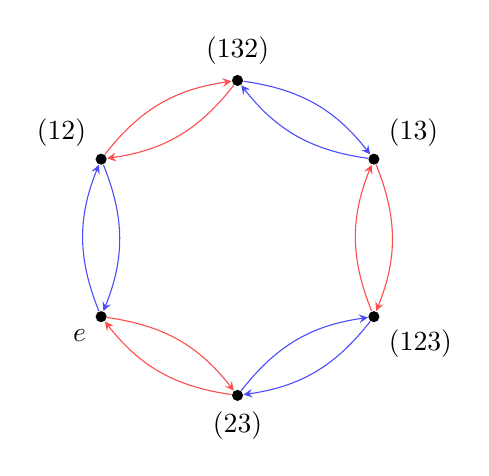
\begin{tikzpicture}
    \pgfmathsetmacro{\len}{2}
    \node[vertex,label=30:$(13)$]   (n13)  at (30:\len)  {};
    \node[vertex,label=90:$(132)$]  (n132) at (90:\len)  {};
    \node[vertex,label=150:$(12)$]  (n12)  at (150:\len) {};
    \node[vertex,label=210:$e$]     (ne)   at (210:\len) {};
    \node[vertex,label=270:$(23)$]  (n23)  at (270:\len) {};
    \node[vertex,label=330:$(123)$] (n123) at (330:\len) {};
    \begin{scope}[every to/.style={bend left=22}]
      % generator a is (12)
      \draw[gena] (ne)   to (n12);
      \draw[gena] (n12)  to (ne);
      \draw[gena] (n13)  to (n132);
      \draw[gena] (n132) to (n13);
      \draw[gena] (n123) to (n23);
      \draw[gena] (n23)  to (n123);
      % generator b is (23)
      \draw[genb] (ne)   to (n23);
      \draw[genb] (n23)  to (ne);
      \draw[genb] (n13)  to (n123);
      \draw[genb] (n123) to (n13);
      \draw[genb] (n12)  to (n132);
      \draw[genb] (n132) to (n12);
    \end{scope}
  \end{tikzpicture}
  \end{sidecaption}
\end{figure}

$G \equiv \Aut(D_G) \to \Sym(\Card G)$

\section{Actions}
\label{sec:actions}

If $G$ is any (possibly higher) group and $A$ is any type of objects,
then we define an \emph{action} by $G$ in the world of elements of $A$ as a function
\[
  X : \BG \to A.
\]
The particular $A$ being acted on is $X(\pt):A$,
and the action itself is given by transport.
This generalizes our earlier definition of $G$-sets, $X : \BG \to \Set$.

Notice that the type $\BG \to A$ is equivalent to the type
\[
  \sum_{a:A}\hom(G,\Aut_A(a)),
\]
that is, the type of pairs of an element $a : A$,
and a homomorphism from $G$ to the automorphism group of $A$.
The equivalence maps $X:\BG\to A$ to the pair consisting of $X(\pt)$
and the homomorphism represented by the pointed map arising
from corestricting $X$ to factor through the component of $A$ containing $a$
together with the trivial proof that this map takes $\pt:\BG$ to $a$.

Because of this equivalence,
we define a \emph{$G$-action on $a:A$}
to be a homomorphism from $G$ to $\Aut_A(a)$.

Many times we are particularly interested in actions on types,
i.e., $A$ is a universe (or the universe of types-at-large):
\[
  X : \BG \to \UU.
\]

In this case, we define \emph{orbit type} of the action as
\[
  X_G \defeq \sum_{z:\BG} X(z),
\]
and the type of \emph{fixed points} as
\[
  X^G \defeq \prod_{z:\BG} X(z).
\]
The set of orbits is the set-truncation of the orbit type,
\[
  X / G \defeq \Trunc{X_G}_0.
\]
We say that the action is \emph{transitive} if $X / G$ is contractible.

\section{Semidirect products}
\label{sec:Semidirect-products}

In this section we describe a generalization of the product of two group, called the {\em semidirect} product, which can be constructed from an
action of a group on a group.  Like the product, it consists of pairs, both at the level of concrete groups and of abstract groups, as we shall
see.

We start with some preliminaries on paths between pairs. 
Lemma \cref{lem:isEq-pair=} above takes a simpler form when $y$ and $y'$ are values of a section $f$ of the family $Y$, as the following lemma shows.

\begin{lemma}\label{lem:pathpairsection}
  Suppose we are given a type $X$ and a family of types $Y(x)$ parametrized by the elements $x$ of $X$.
  Suppose we are also given a section $f : \prod_{x:X} Y(x)$.
  For any elements $x$ and $x'$ of $X$,
  there is an equivalence of type
  $$\left ( (x,f(x)) = (x',f(x')) \right ) \weq (x=x') \times (f(x) = f(x)),$$
  where the identity type on the left side is between elements of $\sum_{x:X} Y(x)$.
\end{lemma}

\begin{proof}
  By \cref{lem:isEq-pair=} and by composition of equivalences, it suffices to establish an equivalence of type
  $$\left( \sum_{p:x=x'} \pathover {f(x)} Y p {f(x')} \right) \weq (x=x') \times (f(x) = f(x)).$$
  Rewriting the right hand side as a sum over a constant family, it suffices to find an equivalence of type
  $$\left( \sum_{p:x=x'} \pathover {f(x)} Y p {f(x')} \right) \weq \sum_{p:x=x'} (f(x) = f(x)).$$
  By \cref{lem:fiberwise} it suffices to establish an equivalence of type 
  $$ \left( \pathover {f(x)} Y p {f(x')} \right) \weq (f(x) = f(x))$$
  for each $p:x=x'$.  By induction on $x'$ and $p$ we reduce to the case where $x'$ is $x$ and $p$ is $\refl x$, and it suffices to establish an
  equivalence of type 
  $$ \left( \pathover {f(x)} Y {\refl x} {f(x)} \right) \weq (f(x) = f(x)).$$
  Now the two sides are equal by definition, so the identity equivalence provides what we need.  
\end{proof}

The lemma above shows how to rewrite certain paths between pairs as pairs of paths.  Now we wish to establish the formula for composition of
paths, rewritten in terms of pairs of paths, but first we introduce a convenient definition for the transport of loops in $Y(x)$ along paths in
$X$.

\begin{definition}\label{def:pathsectionaction}
  Suppose we are given a type $X$ and a family of types $Y(x)$ parametrized by the elements $x$ of $X$.
  Suppose we are also given a section $f : \prod_{x:X} Y(x)$.
  For any elements $x$ and $x'$ of $X$ and for any identity $p : x = x'$, define a function $(f(x') = f(x')) \to (f(x) = f(x))$, to be denoted
  by $q' \mapsto q' \star p$, by induction on $p$ and $x'$, reducing to the case where $x'$ is $x$ and $p$ is $\refl x$, allowing us to
  set $q' \star \refl x \defeq q'$.
\end{definition}  

We turn now to associativity for the operation $\star$.

\begin{lemma}\label{def:pathsectionactionassoc}
  Suppose we are given a type $X$ and a family of types $Y(x)$ parametrized by the elements $x$ of $X$.
  Suppose we are also given a section $f : \prod_{x:X} Y(x)$.
  For any elements $x$, $x'$, and $x''$ of $X$, for any identities $p : x = x'$ and $p' : x' = x''$,
  and for any $q : f x'' = f x''$,
  there is an identity of type $ ( q \star p') \star p = q \star (p' \cdot p)$.
\end{lemma}

\begin{proof}
  By induction on $p$ and $p'$, it suffices to show that $ ( q \star \refl y) \star \refl y = q \star (\refl y \cdot \refl y)$, in which both sides are
  equal to $q$ by definition.
\end{proof}

Observe that the operator $\star$ depends on $f$, but $f$ is not included as part of the notation.

The next lemma contains the formula we are seeking.

\begin{lemma}\label{lem:pathpairsectionmult}
  Suppose we are given a type $X$ and a family of types $Y(x)$ parametrized by the elements $x$ of $X$.
  Suppose we are also given a section $f : \prod_{x:X} Y(x)$.
  For any elements $x$, $x'$, and $x''$ of $X$, and for any two identities $e : (x,f(x)) = (x',f(x'))$ and $e' : (x',f(x')) = (x'',f(x''))$,
  if $e$ corresponds to the pair $(p,q)$ with $p : x = x'$ and $q : f x = f x$ under the equivalence of \cref{lem:pathpairsection},
  and $e'$ corresponds to the pair $(p',q')$ with $p' : x' = x''$ and $q' : f x' = f x'$,
  then $e' \cdot e$ corresponds to the pair $(p' \cdot p , (q' \star p) \cdot q)$.
\end{lemma}

\begin{proof}
  By induction on $p$ and $p'$ we reduce to the case where $x'$ and $x''$ are $x$ and $p$ and $p'$ are $\refl x$. 
  It now suffices to show that $e' \cdot e$ corresponds to the pair $(\refl x , q' \cdot q)$.
  Applying the definition of the map $\Phi$ in the proof of \cref{lem:isEq-pair=} to our three pairs, we see that it suffices to show that
  $\left( \apap g {\refl x} {q'} \right) \cdot \left( \apap g {\refl x} {q} \right) = \apap g {\refl x} {q' \cdot q}$, with $g$, as there, being the function $ g(x)(y) \defeq (x,y)$.
  By \cref{def:applfun2comp} it suffices to show that $\left( \ap {g(x)} {q'} \right) \cdot \left( \ap {g(x)} {q} \right) = \ap {g(x)} {(q' \cdot q)}$, which follows from
  compatibility of $\ap {g(x)}$ with composition, as in \cref{lem:apcomp}.
\end{proof}

The lemma above will be applied mostly in the case where $x'$ and $x''$ are $x$, but if it had been stated only for that case, we would not have
been able to argue by induction on $p$ and $p'$.

\begin{definition}\label{def:semidirect-product}
  Given a group $G$ and an action $\tilde H : \BG \to \typegroup$ on a group $H \defeq \tilde H(\pt)$, we define a group called the {\em
    semidirect product}
  $G \ltimes H$ to be the total space
  $$\clf ( G \ltimes H ) \defeq \sum_{t:\BG} \B \tilde H(t)$$
  equipped with the point $(\sh_G,\pt_H)$ as basepoint and equipped with a proof \cref{lem:UNKNOWN} that it is a connected groupoid.
\end{definition}

The notation $G \ltimes H$, following standard practice, is an abuse, because it includes no reference to the action $\tilde H$, which is needed
to perform the construction.

Projection onto the first factor gives a homomorphism $p : G \ltimes H \to G$, and it has a section $s : G \to G \ltimes H$ provided by the
function $t \mapsto (t,\pt_{\tilde H(t)})$.  The two maps are homomorphisms because they preserve the base points.

%% \begin{exercise}
%%   Construct a section of the projection $ \clf ( G \ltimes H ) \to \BG $ by sending $t$ to $(t,pt)$.
%%   Construct an equivalence between the set $\abstrOp (G \ltimes H)$ and the set $\abstrOp G \times \abstrOp H$.  Use the equivalence to work out
%%   explicit formulas for multiplication and for the inverse operation in the abstract group $\abstrOp (G \ltimes H)$.
%% \end{exercise}

\section{Orbit-stabilizer theorem}
\label{sec:orbit-stabilizer-theorem}

Given an action $X : \BG \to \UU$ and a point $x : X(\pt)$, we define
the \emph{orbit} through $x$ as the subtype of $X(\pt)$ consisting of
all $y : X(\pt)$ that are merely equal to $x$ in the orbit type:
\[
  G\cdot x \defeq \mathcal O_x \defeq \sum_{y : X(\pt)} \merely{[x] = [y]}
\]
(Note the unfortunate terminology: an orbit is not an element in the
orbit type!)
Note that this only depends on the image of $x$ in the set of orbits,
thus justifying the names.

In this way, the type $X(\pt)$ splits as a disjoint union of orbits,
indexed by the set of orbits
\[
  X(\pt) \equiv \coprod_{z : X / G} \mathcal O_z.
\]

The \emph{stabilizer group} $G_x$ of $x : X(\pt)$ is the automorphism group of $[x]$ in the orbit type.
Different points in the same orbit have conjugate stabilizer groups.

We say that the action is \emph{free} if all stabilizer groups are trivial.

\begin{theorem}[Orbit-stabilizer theorem]
  \label{thm:orbitstab}
  Fix a $G$-type $X$ and a point $x : X(\pt)$.
  There is a canonical action $\tilde G : \BG_x \to \UU$,
  acting on $\tilde G(\pt)\equiv G$
  with orbit type $\tilde G\dblslash G_x \equiv \mathcal O_x$.
\end{theorem}
\begin{proof}
  Define $\tilde G(x,y,!) \defeq (\pt = x)$.
\end{proof}

Now suppose that $G$ is a $1$-group acting on a set.
We see that the orbit type is a set
(and is thus equivalent to the set of orbits)
if and only if
all stabilizer groups are trivial,
\ie if and only if the action is free.

If $G$ is a $1$-group,
then so is each stabilizer-group,
and in this case (of a set-action),
the orbit-stabilizer theorem
tells us that 

\begin{theorem}[Lagrange's Theorem]\footnote{insert that the action is free (referred to)}
\label{thm:lagrange}
  If $H \to G$ is a subgroup, then $H$ has a natural action on $G$,
  and all the orbits under this action are equivalent.
\end{theorem}

% Interaction with cardinality: if G acts freely on S, then card(S/G) = card(S)/card(G)

\section{The isomorphism theorems}
\label{sec:noether-theorems}

First a remark about maps between groupoids.
Let $f : X \to Y$, and write $f$ as a projection from a sigma-type:
$\sum_{y:Y} f^{-1}(y) \to Y$,
projecting away the fibers $f^{-1}(y)$.
We say that $f$ \emph{forgets} these fibers.
In general, the fibers are themselves groupoids,
but it can happen that they are sets, propositions, or even contractible.
Accordingly, we say that:
\begin{itemize}
\item $f$ \emph{forgets at most structure} if all the fibers are sets;
\item $f$ \emph{forgets properties} if all the fibers are propositions;
\item $f$ \emph{forgets nothing} if all the fibers are contractible.
\end{itemize}
(Of course, in the latter case, $f$ is an equivalence.)

We can factor $f$ through its $0$- and $-1$-image as follows:
\[
  \sum_{y:Y} f^{-1}(y) \to
  \sum_{y:Y} \Trunc{f^{-1}(y)}_0 \to
  \sum_{y:Y} \Trunc{f^{-1}(y)}_{-1} \to
  \sum_{y:Y} \Trunc{f^{-1}(y)}_{-2} = Y.
\]
Here, the first map \emph{forgets stuff} (it is $0$-connected),
the second map \emph{forgets structure} (it is a $-1$-connected set map),
while the last \emph{forgets properties}.

For example, the inclusion of the type of sets with cardinality
$n$ into the type of all finite sets
forgets properties.

Group homomorphisms provide examples of forgetting stuff and structure.
For example, the map from cyclically ordered sets with cardinality $n$
to the type of sets with cardinality $n$ forgets structure,
and represents an injective group homomorphism from the cyclic
group of order $n$ to the symmetric group $\Sigma_n$.

And the map from pairs of $n$-element sets to $n$-element sets
that projects onto the first factor clearly forgets stuff,
namely, the other component.
It represents a surjective group homomorphism.

More formally, fix two groups $G$ and $H$,
and consider a homomorphism $\varphi$ from $G$ to $H$,
considered as a pointed map $\B\varphi : \BG \to_\pt \BH$.
Then $\B\varphi$ factors as
\begin{align*}
  \BG
  = &\sum_{w:\BH}\sum_{z:\BG}(\B\varphi(z)=w)\\
  \to_\pt &\sum_{w:\BH}\Trunc*{\sum_{z:\BG}(\B\varphi(z)=w)}_0\\
  \to_\pt &\sum_{w:\BH}\Trunc*{\sum_{z:\BG}(\B\varphi(z)=w)}_{-1} = \BH.
\end{align*}
The pointed, connected type in the middle represents a group
that is called the \emph{image} of $\varphi$, $\Img(\varphi)$.


(FIXME: Quotient groups as automorphism groups, normal subgroups/normalizer, subgroup lattice)

\begin{lemma}
  \label{lem:aut-orbit}
  The automorphism group of the $G$-set $G/H$ is isomorphic to $\N_G(H)/H$.
\end{lemma}

\section{(the lemma that is not) Burnside's lemma}
\label{sec:burnsides-lemma}
\label{lem:burnsides-lemma}

\begin{lemma}
  \label{lem:burnside}
  Let $G$ be a finite group acting on a finite set $X$.
  Then the set of orbits is finite with cardinality
  \[
    \Card(X/G) = \frac1{\Card(G)}\sum_{g:\El G}\Card(X^g),
  \]
  where $X^g = \setof{x:X}{gx=x}$ is the set of elements
  that are fixed by $g$.
\end{lemma}
\begin{proof}
  Since $X$ and $G$ is finite, we can decide equality of their elements.
  Hence each $X^g$ is a finite set, and since $G$ is finite,
  we can decide whether $x,y$ are in the same orbit by searching
  for a $g : \El G$ with $gx = y$.
  Hence the set of orbits is a finite set as well.
  
  Consider now the set $R \defeq \sum_{g:\El G} X^g$,
  and the function $q : R \to X$
  defined by $q(g,x) \defeq x$.
  The map $q^{-1}(x) \to G_x$ that sends $(g,x)$ to $g$ is a bijection.
  Thus, we get the equivalences
  \[
    R \jdeq \sum_{g:\El G} X^g \equiv \sum_{x:X} G_x
    \equiv \sum_{z:X/G} \sum_{x : \mathcal O_z} G_x,
  \]
  where the last step writes $X$ as a union of orbits.
  Within each orbit $\mathcal O_z$,
  the stabilizer groups are conjugate,
  and thus have the same finite cardinality,
  which from the orbit-stabilizer theorem (\cref{thm:orbit-stabilizer}),
  is the cardinality of $G$ divided by the cardinality of $\mathcal O_z$.
  We conclude that $\Card(R) = \Card(X/G)\Card(G)$, as desired.
\end{proof}

% Where does this go?!
\section{More about automorphisms}
\label{sec:automorphisms}

% Written to record somewhere the results of a discussion with Bjorn
For every group $G$ (which for the purposes of the discussion
in this section we allow to be a higher group)
we have the automorphism group $\Aut(G)$.
This is of course the group of self-identifications $G = G$ in the type of groups, $\Group$.
If we represent $G$ by the pointed connected classifying type $\BG$,
then $\Aut(G)$ is the type of pointed self-equivalences of $\BG$.

We have a natural forgetful map from groups to the type of connected groupoids.
Define the type $\Bunch$ to be the type of all connected groupoid.
If $X:\Bunch$, then all the elements of $X$ are merely isomorphic,
that is, they all look alike,
so it makes sense to say that $X$ consists of a \emph{bunch} of alike objects.

For every group $G$ we have a corresponding bunch, $\BG_\div$,
\ie{} the collection of $G$-torsors,
and if we remember the basepoint $\pt : \BG_\div$,
then we recover the group $G$.
Thus, the type of groups equivalent to the type
$\sum_{X : \Bunch} X$
of pairs of a bunch together with a chosen element.
(This is essentially our definition of the type $\Group$.)

Sometimes we want to emphasize that we $\BG_\div$ is a bunch,
so we define $\bunch(G) \defeq \BG_\div : \Bunch$.

\begin{definition}[The center as an abelian group]
  \label{def:center}
  Let $Z(G) \defeq \prod_{z : \BG}(z = z)$ denote the type of fixed points of the adjoint action of $G$ on itself.
  This type is equivalent to the automorphism group of the identity on $\bunch(G)$,
  and hence the loop type of
  \[
    \B Z(G) \defeq \sum_{f : \BG \to \BG} \merely{f \sim \id}.
  \]
  This type is itself the loop type of the pointed, connected type
  \[
    \B^2Z(G) \defeq \sum_{X : \Bunch}\Trunc{\bunch(G) = X}_0,
  \]
  and we use this to give $Z(G)$ the structure of an \emph{abelian} group,
  called the \emph{center} of $G$.
\end{definition}
There is a canonical homomorphism from $Z(G)$ to $G$ given by the pointed map
from $\B Z(G)$ to $\BG$ that evaluates at the point $\pt$.
The fiber of the evaluation map $e : \B Z(G) \to_\pt \BG$ is
\begin{align*}
  \fiber_e(\pt)
  &\jdeq \sum_{f : \BG \to \BG} \merely{f \sim \id} \times (\mathop f \pt = \pt) \\
  &\equiv \sum_{f : \BG \to_\pt \BG} \merely{f \sim \id},
\end{align*}
and this type is the loop type of the pointed, connected type
\[
  \B\Inn(G) \defeq \sum_{H : \Group} \Trunc{\bunch(G) = \bunch(H)}_0,
\]
thus giving the homomorphism $Z(G)$ to $G$ a normal structure with
quotient group $\Inn(G)$, called the \emph{inner automorphism group}.

Note that there is a canonical homomorphism from $\Inn(G)$ to $\Aut(G)$
given by the pointed map $i : \B\Inn(G) \to \B\Aut(G)$ that forgets the component.
On loops, $i$ gives the inclusion into $\Aut(G)$ of the subtype of automorphisms of $G$
that become merely equal to the identity automorphism of $\bunch(G)$.
The fiber of $i$ is
\begin{align*}
  \fiber_i(\pt)
  &\jdeq \sum_{H : \Group} \Trunc{\bunch(G) = \bunch(H)}_0 \times (H = G) \\
  &\equiv \Trunc{\bunch(G) = \bunch(G)}_0.
\end{align*}
This is evidently the type of loops in the pointed, connected groupoid
\[
  \B\Out(G) \defeq \Trunc*{\sum_{X : \Bunch}\merely{\bunch(G) = X}}_1,
\]
thus giving the homomorphism $\Inn(G)$ to $\Aut(G)$ a normal structure with
quotient group $\Out(G)$, called the \emph{outer automorphism group}.
Note that $\Out(G)$ is always a $1$-group,
and that it is the decategorification of $\Aut(\bunch(G))$.

\begin{theorem}
  Let two groups $G$ and $H$ be given.
  There is a canonical action of $\Inn(H)$
  on the set of homomorphisms from $G$ to $H$, $\Trunc{\BG \to_\pt \BH}_0$.
  This gives rise to an equivalence
  \[
    \Trunc{\BG_\div \to \BH_\div}_0 \equiv \Trunc*{\Trunc{\BG \to_\pt \BH}_0 \dblslash \Inn(H)}_0
  \]
  between the set of maps from $\bunch(G)$ to $\bunch(H)$ and the set of
  components of the orbit type of this action.
\end{theorem}
\begin{proof}
  We give the action by defining a type family $X : \B\Inn(H) \to \UU$ as follows
  \[
    X\, \angled{K,\phi} \defeq \Trunc{\Hom(G,K)}_0 \jdeq \Trunc{\BG \to_\pt \BK}_0,
  \]
  for $\angled{K,\phi} : \B\Inn(H) \jdeq \sum_{K : \Group} \Trunc{\bunch(H) = \bunch(K)}_0$.
  Now we can calculate
  \begin{align*}
    \Trunc{X_{\Inn(H)}}_0
    &\jdeq \Trunc*{\sum_{K:\Group}\Trunc{\bunch(H)=\bunch(K)}_0\times\Trunc{\Hom(G,K)}}_0 \\
    &\equiv \Trunc*{\sum_{K:\Group}(\bunch(H)=\bunch(K))\times\Hom(G,K)}_0 \\
    &\equiv \Trunc*{\sum_{K:\Bunch}\sum_{k:K}(\bunch(H)=K)\times\sum_{f:\bunch(G)\to K)}\mathop f \pt = k}_0 \\
    &\equiv \Trunc*{\sum_{K:\Bunch} (\bunch(H)=K) \times(\bunch(G) \to K)}_0 \\
    &\equiv \Trunc*{\bunch(G)\to\bunch(H)}_0 \jdeq \Trunc*{\BG_\div \to \BH_\div}_0.\qedhere
  \end{align*}
\end{proof}

\section{Orbit type as a groupoid completion(*)}

\emph{This is a somewhat advanced topic that should occur much later, if at all.}

\bigskip

Suppose $G$ is a group acting on a groupoid $X$,
given by a map $X : \BG \to_\pt \B\!\Aut(X_0)$,
with $e_X : X(\pt) = X_0$.
By induction on $e_X$ we may assume that $X_0\jdeq X(\pt)$
and $e_X\jdeq\refl{}$.

We have the orbit type $X\dblslash G \jdeq \sum_{T:\BG}X(T)$.
We think of this as identifying elements of $X_0$
that are in the same orbit,
in the sense that there are new identifications of $x$ and $y$
for group elements $g$ with $g\cdot x = y$.

In this section we study one way of making this intuition precise.

Consider the pregroupoid $C_G(X)$ with object type $X_0$ and morphism sets
\[
  \hom(x,y) \defeq \sum_{g:G}(g\cdot x = y),
\]
where $g\cdot x \defeq g_*(x)$. The identity at $x$ is
$(1,\id)$, while the composite of $(g,p):\hom(x,y)$ with
$(h,q):\hom(y,z)$ is $(hg,r)$, where $r$ is built from $p$ and $q$ as
follows:
\[
  hg \cdot x = h\cdot(g\cdot x) = h\cdot y = z.
\]

We have a functor of pregroupoids $F: C_G(X) \to X \dblslash G$
defined on objects by
$F(x) := (\pt,x)$ and on morphisms $(g,p):\hom(x,y)$ by $F(g,p) :=
(g,p)^=$.

This functor is essentially surjective on objects (by connectivity of
$\BG$) and fully faithful by the characterization of paths in
$\sum$-types. Hence it induces an equivalence from the completion of
$C_G(X)$ to $X\dblslash G$.

As a corollary, the orbit set $X/G \jdeq \Trunc{X \dblslash G}_0$,
is the set quotient of $X_0$ modulo the equivalence relation
$x \sim y \defeq \exists g:G, g\cdot x = y$.

%%% Local Variables:
%%% mode: latex
%%% fill-column: 144
%%% TeX-master: "book"
%%% End:
